\begin{figure}[htbp]
\centering
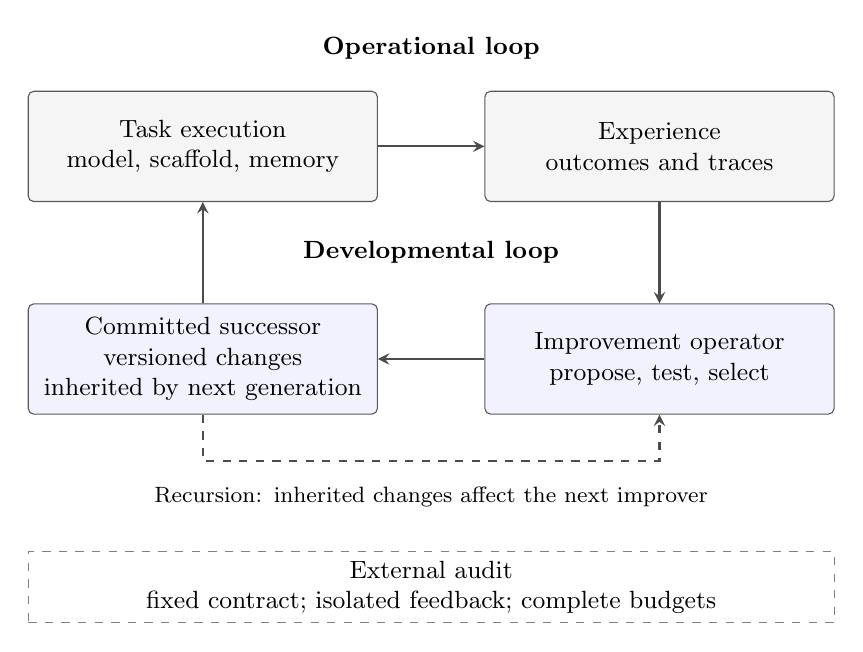
\begin{tikzpicture}[>=stealth, every node/.style={font=\small},
box/.style={draw=black!65, rounded corners=2pt, align=center, minimum height=1.4cm, text width=4.2cm},
arr/.style={->,thick,draw=black!70}]
\node[font=\small\bfseries] at (2.9,1.25) {Operational loop};
\node[box,fill=black!4] (task) at (0,0) {Task execution\\model, scaffold, memory};
\node[box,fill=black!4] (evidence) at (5.8,0) {Experience\\outcomes and traces};
\node[font=\small\bfseries] at (2.9,-1.35) {Developmental loop};
\node[box,fill=blue!5] (improver) at (5.8,-2.7) {Improvement operator\\propose, test, select};
\node[box,fill=blue!5] (commit) at (0,-2.7) {Committed successor\\versioned changes\\inherited by next generation};
\draw[arr] (task)--(evidence);
\draw[arr] (evidence)--(improver);
\draw[arr] (improver)--(commit);
\draw[arr] (commit)--(task);
\draw[arr,dashed] (commit.south) -- (0,-4.0) -- (5.8,-4.0) -- (improver.south);
\node[align=center,text width=10cm,font=\footnotesize] at (2.9,-4.45) {Recursion: inherited changes affect the next improver};
\node[draw=black!50,dashed,align=center,text width=10cm,minimum height=0.85cm] at (2.9,-5.6) {External audit\\fixed contract; isolated feedback; complete budgets};
\end{tikzpicture}
\caption{Two coupled loops and the additional inheritance relation needed for a recursive claim. The external audit is an experimental boundary in the proposed evaluation protocol. This diagram is the survey's synthesis, not a reproduced figure.}
\label{fig:loops}
\end{figure}
